% Choose one to switch between slides and handout
%\documentclass[]{beamer}
\documentclass[handout]{beamer}

% Video Meta Data
\title{Bitcoin, Blockchain and Cryptoassets}
\subtitle{Bitcoin Pricing Models}
\author{Prof. Dr. Fabian Schär}
\institute{University of Basel}

% Config File
% Packages
\usepackage[utf8]{inputenc}
\usepackage{hyperref}
\usepackage{gitinfo2}
\usepackage{tikz}
\usepackage{amsmath}
\usepackage{mathtools}
\usepackage{bibentry}
\usepackage{xcolor}
\usepackage{colortbl} % Add colour to LaTeX tables
\usepackage{caption}
\usepackage[export]{adjustbox}
\usepackage{pgfplots} \pgfplotsset{compat = 1.17}
\usepackage{makecell}
\usepackage{fancybox}
\usepackage{ragged2e}
\usepackage{fontawesome}
\usepackage{seqsplit}
\usepackage{tabularx}

% Color Options
\definecolor{highlight}{rgb}{0.65,0.84,0.82}
\definecolor{focus}{rgb}{0.72, 0, 0}
\definecolor{lightred}{rgb}{0.8,0.5,0.5}
\definecolor{midgray}{RGB}{190,195,200}

% Beamer Template Options
\beamertemplatenavigationsymbolsempty
\setbeamertemplate{footline}[frame number]
\setbeamercolor{structure}{fg=black}
\setbeamercolor{footline}{fg=black}
\setbeamercolor{title}{fg=black}
\setbeamercolor{frametitle}{fg=black}
\setbeamercolor{item}{fg=black}
\setbeamercolor{}{fg=black}
\setbeamercolor{bibliography item}{fg=black}
\setbeamercolor*{bibliography entry title}{fg=black}
\setbeamercolor{alerted text}{fg=focus}
\setbeamertemplate{items}[square]
\setbeamertemplate{enumerate items}[default]
\captionsetup[figure]{labelfont={color=black},font={color=black}}
\captionsetup[table]{labelfont={color=black},font={color=black}}

\setbeamertemplate{bibliography item}{\insertbiblabel}

% Link Icon Command
\newcommand{\link}{%
    \tikz[x=1.2ex, y=1.2ex, baseline=-0.05ex]{%
        \begin{scope}[x=1ex, y=1ex]
            \clip (-0.1,-0.1)
                --++ (-0, 1.2)
                --++ (0.6, 0)
                --++ (0, -0.6)
                --++ (0.6, 0)
                --++ (0, -1);
            \path[draw,
                line width = 0.5,
                rounded corners=0.5]
                (0,0) rectangle (1,1);
        \end{scope}
        \path[draw, line width = 0.5] (0.5, 0.5)
            -- (1, 1);
        \path[draw, line width = 0.5] (0.6, 1)
            -- (1, 1) -- (1, 0.6);
        }
    }

% Read Git Data from Github Actions Workflow
% Defaults to gitinfo2 for local builds
\IfFileExists{gitInfo.txt}
	{\input{gitInfo.txt}}
	{
		\newcommand{\gitRelease}{(Local Release)}
		\newcommand{\gitSHA}{\gitHash}
		\newcommand{\gitDate}{\gitAuthorIsoDate}
	}

% Custom Titlepage
\defbeamertemplate*{title page}{customized}[1][]
{
  \vspace{-0cm}\hfill\includegraphics[width=2.5cm]{../config/logo_cif}
  \includegraphics[width=1.9cm]{../config/seal_wwz}
  \\ \vspace{2em}
  \usebeamerfont{title}\textbf{\inserttitle}\par
  \usebeamerfont{title}\usebeamercolor[fg]{title}\insertsubtitle\par  \vspace{1.5em}
  \small\usebeamerfont{author}\insertauthor\par
  \usebeamerfont{author}\insertinstitute\par \vspace{2em}
  \usebeamercolor[fg]{titlegraphic}\inserttitlegraphic
    \tiny \noindent \texttt{Release Ver.: \gitRelease}\\ 
    \texttt{Version Hash: \gitSHA}\\
    \texttt{Version Date: \gitDate}\\ \vspace{1em}
    
    
    \iffalse
  \link \href{https://github.com/cifunibas/Bitcoin-Blockchain-Cryptoassets/blob/main/slides/intro.pdf}
  {Get most recent version}\\
  \link \href{https://github.com/cifunibas/Bitcoin-Blockchain-Cryptoassets/blob/main/slides/intro.pdf}
  {Watch video lecture}\\ 
  
  \fi
  
  \vspace{1em}
  License: \texttt{Creative Commons Attribution-NonCommercial-ShareAlike 4.0 International}\\\vspace{2em}
  \includegraphics[width = 1.2cm]{../config/license}
}


% tikzlibraries
\usetikzlibrary{decorations.pathreplacing}
\usetikzlibrary{decorations.markings}
\usetikzlibrary{positioning}
\usetikzlibrary{calc}
\captionsetup{font=footnotesize}


%%%%%%%%%%%%%%%%%%%%%%%%%%%%%%%%%%%%%%%%%%%%%%
%%%%%%%%%%%%%%%%%%%%%%%%%%%%%%%%%%%%%%%%%%%%%%
\begin{document}

\thispagestyle{empty}
\begin{frame}[noframenumbering]
	\titlepage
\end{frame}

\begin{frame}{Recap: Monetary Value}
	\begin{table}[h]
		\begin{center}
			\begin{tabular}{rl}
				\hline \hline
  					& \text{Intrinsic value}\\
				\text{+} & \text{Promise of payment}\\
				\text{+} & \text{Liquidity premium}\\
				\hline
				\text{=} & \text{Market value of monetary unit}\\
				\hline \hline
			\end{tabular}
		\end{center}
	\end{table}
	\vspace{1.5em}
	\uncover<2->{$\rightarrow$ Bitcoin's value is solely determined by its liquidity premium.}
\end{frame}

\begin{frame}{Discounted Cash Flow (DCF)}
	\begin{equation}
		DCF = \frac{CF_1}{(1 + r)^1} + \frac{CF_2}{(1 + r)^2} + \dots + \frac{CF_n}{(1 + r)^n}	\end{equation}
	
	\vspace{1.5em}
	
	\begin{columns}
		\uncover<2->{
			\begin{column}{0.5\textwidth}
				\begin{figure}
					\includegraphics[width = 0.3\textwidth]{../assets/images/firm.png}
					\caption*{Cash flows}
				\end{figure}
			\end{column}
			}
		\uncover<3->{	
			\begin{column}{0.5\textwidth}
				\begin{figure}
					
\includegraphics[width = 0.3\textwidth]{../assets/images/bitcoin.png}	
					\caption*{Cash flows?}
				\end{figure}
			\end{column}
		}
	\end{columns}
\end{frame}

\begin{frame}{Stock-to-Flow}
	\begin{figure}
		\input{../assets/figures/stock_to_flow.tex}	
	\end{figure}
	\vspace{1em}
	\begin{columns}[T]
		\begin{column}{0.5\textwidth}
			\uncover<2->{
				\begin{equation}
					SF_{t+1} = \frac{M_t}{M_{t+1} -  M_t}	
				\end{equation}
			}
		\end{column}
		\begin{column}{0.5\textwidth}
			\uncover<3->{
				\begin{equation}
					g_{t+1} = \frac{M_{t+1} - M_t}{M_t}
				\end{equation}
			}
		\end{column}
	\end{columns}
\end{frame}

\begin{frame}{Bitcoin Supply}
	\begin{figure}
		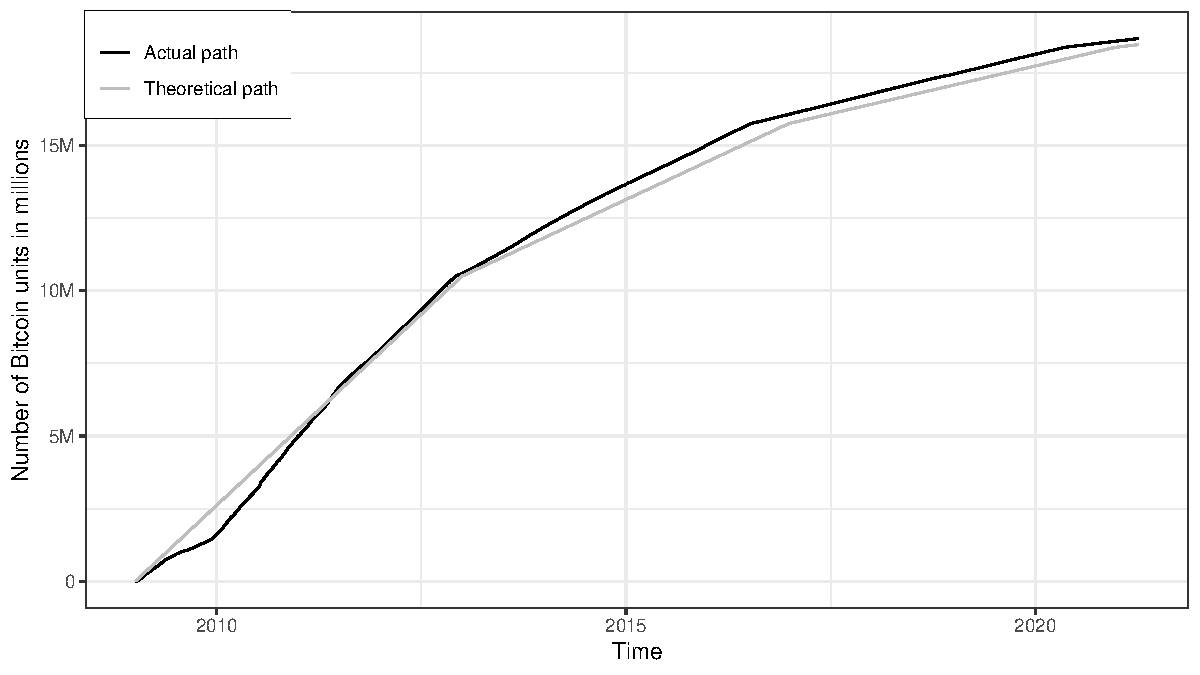
\includegraphics[width = 0.9\textwidth]{../assets/figures/mined_theoretical_btc}
	\caption*{\textit{Data source:} blockchain.info}
	\end{figure}
\end{frame}

\begin{frame}{Growth Rate of the Monetary Supply}
	\begin{figure}
		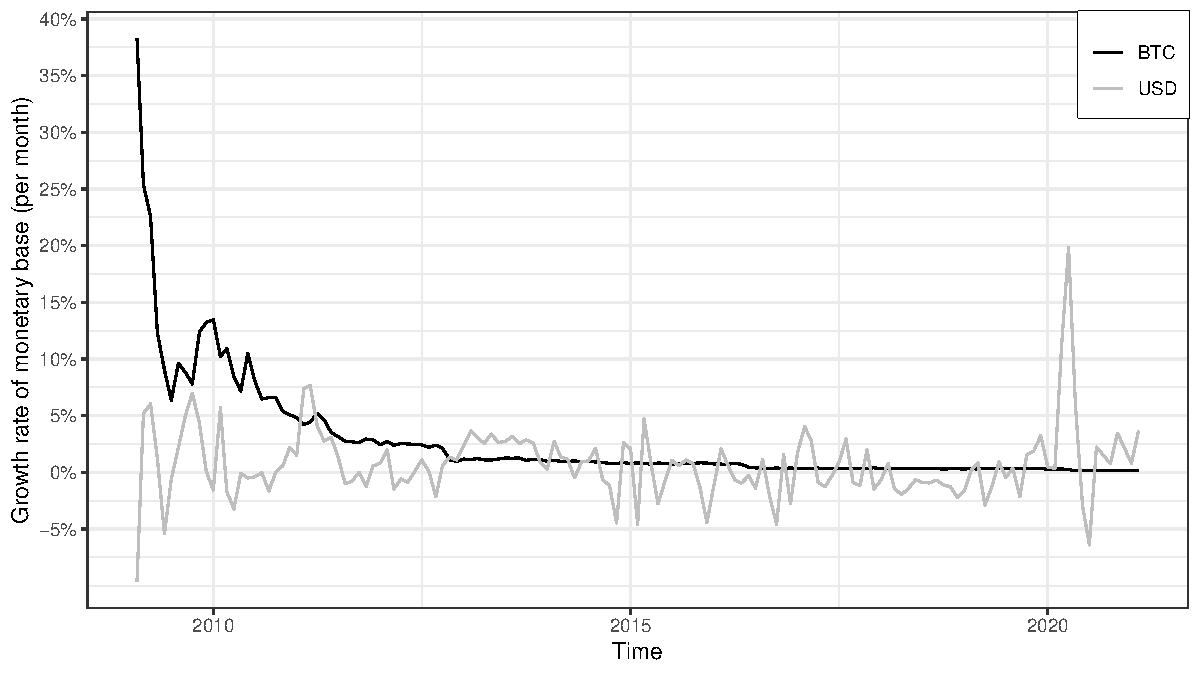
\includegraphics[width = 0.9\textwidth]{../assets/figures/btc_usd_growth.pdf}
	\caption*{\textit{Data sources:} blockchain.info and FRED}
	\end{figure}
\end{frame}

\begin{frame}{Growth Rate of the Monetary Supply}
	\begin{figure}
		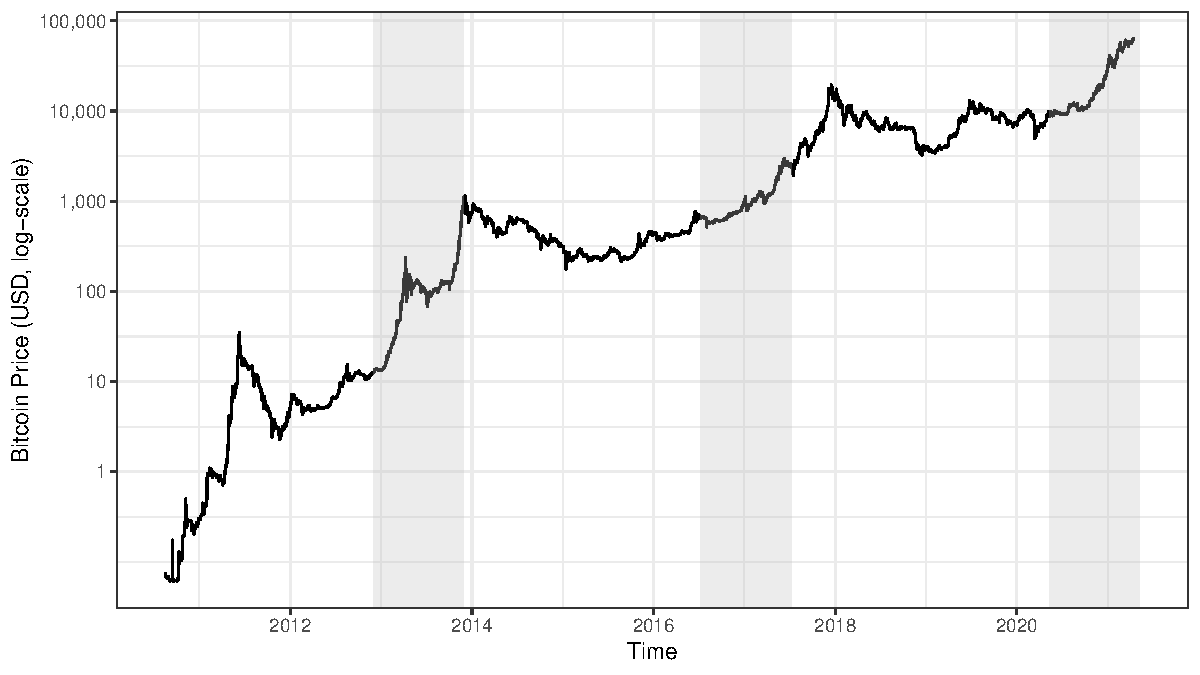
\includegraphics[width = 0.9\textwidth]{../assets/figures/log_price_halvings_graph.pdf}
	\caption*{\textit{Price data sources:} blockchain.info and coinmarketcap.com}
	\end{figure}
\end{frame}

\begin{frame}{Price Expectations}
	\textbf{Is Bitcoin deflationary?}\\
	\begin{columns}
		\begin{column}{0.5\textwidth}
			\begin{figure}
				\input{../assets/figures/btc_supply_demand.tex}	
			\end{figure}
		\end{column}
		\begin{column}{0.5\textwidth}
			\begin{itemize}
				\item<2-> Ever-increasing demand?
				\item<3-> Limited (even decreasing?) total supply
			\end{itemize}
		\end{column}
	\end{columns}
	\vspace{0.5em}
	\uncover<4->{
		\textbf{Will the value increase forever?}\\
		\begin{columns}
			\begin{column}{0.5\textwidth}
				\uncover<5->{
					\begin{figure}
						\input{../assets/figures/expectations.tex}	
					\end{figure}
				}
			\end{column}
			\begin{column}{0.5\textwidth}
				\uncover<5->{
					Two equilibria:\\
					\begin{itemize}
						\item $p = 0$
						\item $p > 0$
					\end{itemize}
				}
			\end{column}
		\end{columns}
	}
\end{frame}

\begin{frame}[fragile]{Bitcoin as a Store of Value}
	\begin{quote}{''As a thought experiment, imagine there was a base metal as scarce as gold but with the following properties:\\
	- boring grey in colour\\
	- not a good conductor of electricity\\
	- not particularly strong, but not ductile or easily malleable either\\
	- not useful for any practical or ornamental purpose\\
\hfill \\
	and one special, magical property:\\
	- can be transported over a communications channel"
		}
	\end{quote}

	\textit{Source:} \href{https://bitcointalk.org/index.php?topic=583.msg11405#msg11405}{\link satoshi on bitcointalk.org}
\end{frame}

\end{document}